\chapter{Realizability Problems for Weighted Trees}\label{chp:disk}

In this chapter our goal is to prove Theorem \ref{thm:disk} which states: ``It is NP-Hard to decide whether a given tree with positive vertex weights is the contact graph of a disk arrangements with specified radii.''  
This chapter's approach to proving Theorem \ref{thm:disk} introduces an ordered weighted tree $T$ and perturbed ordered weight tree $T_\epsilon$, the Hausdorff distance, and then prove the following lemma:
\begin{lem}\label{lem:ch4IntroLemma}
for ever $\epsilon > 0$, there exists an ordered weighted tree $T_\epsilon$ such that every realization of $T_\epsilon$ as an ordered disk contact graph where the radii of the disks equal the vertex weights.
\end{lem} 
Using Lemma \ref{lem:ch4IntroLemma}, we prove Theorem \ref{thm:disk} by extending the modified auxiliary construction in Chapter \ref{chapter:polygonalLinkage}.  

We first cover the preliminary concepts of Hausdorff distance and the ordered weighted tree families of $T$ and $T_\epsilon$.  
We then continue with the proof of Lemma \ref{lem:ch4IntroLemma} and Theorem \ref{thm:disk}.  
%\chapter{Disk Arrangement}
\section{Properties for Weighted Trees and Polygonal Linkages}
In order to perform our analysis for weighted trees and polygonal linkages, we'll want to use a suitable metric.  The usual Euclidian distance will not suffice for this analysis and so we turn to the Hausdorff distance.
\paragraph{Hausdorff Distance}  Let $A$ and $B$ be sets in the plane. The \textit{directed Hausdorff distance} is 
\begin{equation}\label{eqn:ContactGraphV3-1}
d\lr{A,B} = \sup_{a \in A} \inf_{b \in B} \left\vert\left\vert a-b \right\vert \right\vert
\end{equation}
$h\lr{A,B}$ finds the furthest point $a in A$ from any point in $B$.  \textit{Hausdorff distance} is
\begin{equation}\label{eqn:ContactGraphV3-2}
D\lr{A,B} = \max \left\lbrace d\lr{A,B}, d\lr{B,A} \right\rbrace
\end{equation}
\begin{figure}[!htbp]
\begin{center}
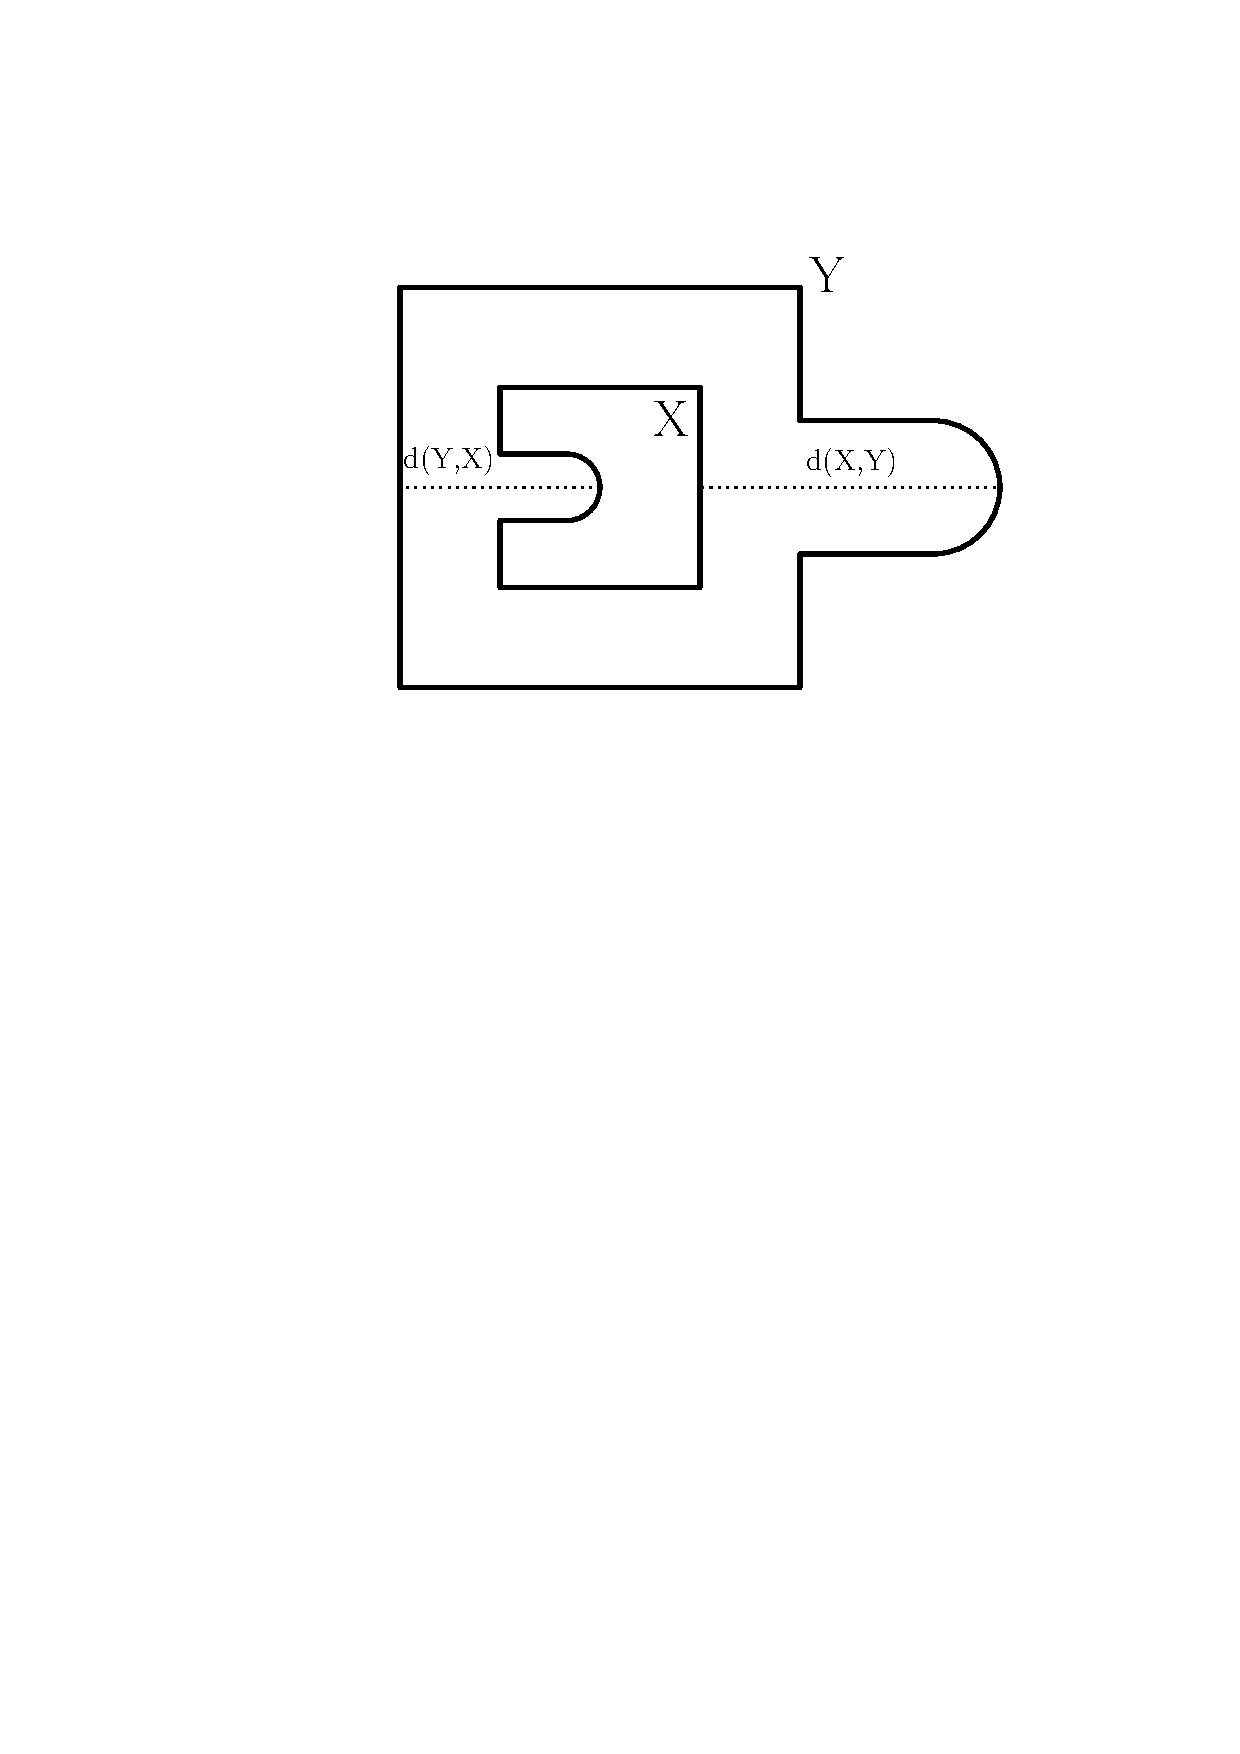
\includegraphics[scale=.5]{graphics/HausdorffDistanceExample1.pdf}
\caption{An illustrative example of $d(X,Y)$ and $d(Y,X)$ where $X$ is the inner curve, and $Y$ is the outer curve.}\label{fig:HausdorffDistanceExample1.pdf}
\end{center}
\end{figure}
\paragraph{$\epsilon$-approximation}
% Modeling the logic engine with polygonal linkages requires reflected copies of the
% rectangles. For an oriented realization, we use a different technique in Section 3. The
% above proof can be adapted to the realization of contact trees of disks by approximating
% rectangles with disk arrangements. In this context, we say that a weighted graph G is a
% ε-approximation of a polygon P if G is realizable as a contact graph of disks of given
% radii, and in every such realization, the Hausdorff distance between the union of disks
% and a congruent copy of P is at most ε. A weighted graph G is a stable ε-approximation
% if, in addition, for every two such realizations of G, the distance between the centers of
% the corresponding disks is at most ε after a suitable rigid transformation.
The weighted graph, $G$, is an \textit{$\epsilon$-approximation} of a polygon $P$ if the Hausdorff distance between every realization such realization of $G$ as a contact graph of disks and a congruent copy of $P$ is at most epsilon.  A weighted graph $G$ is said to be a \textit{$\BigOh{f(x)}$-approximation} of a polygon P if there is a positive constant $M$ such that for all sufficiently large values of $x$ the Hausdorff distance between every realization such realization of $G$ as a contact graph of disks and a congruent copy of $P$ is at $M \cdot \vert f(x)\vert$. A weighted graph $G$ is said to be a \textit{stable} if it has the property that for every two such realizations of $G$, the distance between the centers of the corresponding disks is at most $\epsilon$ after a suitable rigid transformation.  
\section{Weight Trees $T_k$}
In this section we describe a particular family of unit weight trees and corresponding contact graphs disk arrangements called \textit{snowflakes}.  
Note that we regard snowflakes with unit weight as a weight of $\frac{1}{2}$.  
For $i \in \bbN$, the construction of the snowflake tree, $T_i$, is as follows:
\begin{itemize}
\item Let $v_0$ be a dvertex that has six paths attached to it: $p_1$, $p_2$, $\dots$, $p_6$.  Each path has $i$ vertices.
\item For every other path $p_1$, $p_3$, and $p_5$: 
	\begin{itemize}
		\item 	Each vertex on that path has two paths attached, one path on each side of $p_k$.
		\item	The number of vertices that lie on a path attached to the $j^\text{th}$ vertex of $p_k$ is $i-j$.
	\end{itemize}
\end{itemize}

\begin{figure}[!htbp]
\begin{center}
\includegraphics{graphics/snowflakeOutline5LayerSmall.pdf}
\caption{The same contact graph as in figure \ref{fig:hexagonOutline5LayerSmall.pdf} overlayed with the a perfectly weighted snowflake tree.}\label{fig:snowflakeOutline5LayerSmall.pdf}
\end{center}
\end{figure}

A \textit{perfectly weighted snowflake tree} is a snowflake tree with all vertices having weight $\frac{1}{2}$.   
A \textit{perturbed snowflake tree} is a snowflake tree with all vertices having weight of 1 with the exception of $v_0$;  in a perturbed snowflake tree, $v_0$ will have a weight of $\frac{1}{2} + \gamma$.  
For our analysis, all realizations of any snowflake, perfect or perturbed, shall have $v_0$ fixed at origin.  
% This is said to be the canonical position under Hausdorff distance of the snowflake tree.   

\paragraph{Perfectly Weighted Snowflake Tree.}

Consider the graph of the triangular lattice with unit distant edges:
\begin{eqnarray*}
V &=& \left\lbrace a\cdot (1,0) + b \cdot \left(\frac{1}{2},\frac{\sqrt{3}}{2}\right) : a,b \in \bbZ \right\rbrace\\
E &=& \left\lbrace \left\lbrace u,v \right\rbrace : \vert\vert u-v \vert\vert = 1 \text{ and } u,v \in V\right\rbrace
\end{eqnarray*}
The following graph, $G=(V,E)$ is said to be the \textit{unit distance graph} of the triangular lattice.  
We can show that no two distinct edges of this graph are non-crossing.  
First suppose that there were two distinct edges that crossed, $\left\lbrace u_1,v_1 \right\rbrace $ and $\left\lbrace u_2,v_2 \right\rbrace$.  
With respect to $u_1$, there are 6 possible edges corresponding to it, with each edge $\frac{\pi}{3}$ radians away from the next.  
Neither edge crosses another; and so we have a contradiction that there are no edge crossings with $\left\lbrace u_1,v_1 \right\rbrace $.  


The perfectly weighted snowflake tree that is a subgraph over the \textit{unit distance graph}, $G=(V,E)$, of the triangular lattice.  
To show this, for any $S_i$, fix $v_0 = 0 \cdot \cdot (1,0) + 0 \cdot \left(\frac{1}{2},\frac{\sqrt{3}}{2}\right)=\lr{0,0} \in V$ at origin.  
Next consider the six paths attached from origin.  
Fix each consecutive path $\frac{\pi}{3}$ radians away from the next such that the following points like on the corresponding paths: $\lr{1,0} \in p_1, \lr{\frac{1}{2} ,\frac{\sqrt{2}}{3}} \in p_2,\lr{-\frac{1}{2}\p_4,\frac{\sqrt{3}}{2}} \in p_3, \lr{-1,0} \in p4, \lr{-\frac{1}{2},-\frac{\sqrt{3}}{2}}\in p_5,\lr{\frac{1}{2},-\frac{\sqrt{3}}{2}}\in p_6$.  
For $S_i$, there are $i$ vertices on each path.  

We define the six paths from origin as follows:      
\begin{eqnarray*}
p_1 &=& \set{a\cdot\lr{1,0} = \vec{v}}{a \in \bbR^+}\\
p_2 &=& \set{a\cdot\lr{\frac{1}{2},\frac{\sqrt{3}}{2}} = \vec{v}}{a \in \bbR^+}\\
p_3 &=& \set{-a\cdot \lr{1,0} + a \cdot \lr{\frac{1}{2},\frac{\sqrt{3}}{2}} = a\lr{-\frac{1}{2},\frac{\sqrt{3}}{2}} = \vec{v}}{a \in \bbR^+}\\
p_4 &=& \set{a \cdot \lr{-1,0} = \vec{v}}{a \in \bbR^+}\\
p_5 &=& \set{a \cdot \lr{-\frac{1}{2},-\frac{\sqrt{3}}{2}}  = \vec{v}}{a \in \bbR^+}\\
p_6 &=& \set{ a\cdot \lr{1,0} - a \cdot \lr{\frac{1}{2},\frac{\sqrt{3}}{2}}= a \cdot \lr{\frac{1}{2}, -\frac{\sqrt{3}}{2}}}{a \in \bbR^+} 
\end{eqnarray*}
For $S_i$ there exists $i$ vertices on each path.  We shall denote the $\ith$ vertex on the $\jth$ path as $v_{j,i}$.  
For each path defined above, the paths are defined as a set of vectors, $\vec{v} = a \cdot \vec{p}$  for some $a \in \bbR^+$ and $\vec{p} \in \bbR^2$.  
By setting $a = 1,2,\dots, i$, we obtain points that are contained in $V$.  
For $j = 1$, $3$, $5$ and $l = 3 b \leq i$ where $b \in \bbN$,  there exists two paths attached to each vertex $v_{j,l}$.  
We borrow the term \textit{petiole} from botany to describe the two paths attached to $v_{j,l}$.  
In botany, the stalk that attaches to a stem of a plant is called a petiole; petioles usually have leaves attached to their ends.  
For $S_i$, each petiole attached to the $k^\text{th}$ vertex of $p_j$, there are $i-k$ vertices. 
For each vertex $v$ on a petiole, which is not in the paths $p_1$, $p_3$, or $p_5$, there are two \textit{leafs} on either side of the vertex; each leaf is a vertex that has an edge with $v$.  
The one exception to the two leafs rule is on the first vertex of the petiole off of $p_1$, $p_3$, or $p_5$.  
In this exception, attach one leaf to the side of the vertex that is closest to center vertex $v_0$.

The triangular lattice is symmetric under rotation about $v_0$ by $\frac{\pi}{3}$ radians.  
For each vertex $v_{1,l}$ and $l = 3 b \leq i$ where $b \in \bbN$, we place two petioles from it; the first petiole $\frac{\pi}{3}$ above $p_1$ at $v_{1,l}$ and $\frac{-\pi}{3}$ below $p_1$ at $v_{1,l}$ and call these petioles $p_{1,l}^+$ and $p_{1,l}^-$ respectively.  
With respect to $v_{1,l}$, one unit along $p_{1,l}^+$ is a point on the triangular lattice and similarly so on $p_{1,l}^-$.  
Continuing the walk along these paths, unit distance-by-unit distance, we obtain the next point corresponding point on the the triangular lattice up to $i-k$ distance away from $v_{1,l}$.  
Without loss of generality, for each each vertex $v$ of the petiole which are not in $p_1$ have two associated leaf nodes $v^+$ and $v^-$; $v^+$ is placed $\frac{\pi}{3}$ and one unit above $v$ and $v^-$ is placed $\frac{-\pi}{3}$ and one unit below $v$.  
Thus all leaf nodes are in the triangular lattics.
This shows that each of the $i-k$ vertices on $p_{1,l}^-$, $p_{1,l}^+$, and leafs are in $V$.
By rotating all of the paths along $p_1$ by $\frac{2\pi}{3}$ and $\frac{4\pi}{3}$, we obtain the the paths along $p_3$ and $p_5$ respectively, completing the construction.

In Figure \ref{fig:hexagonPetiolesLeafs9Layers.pdf}, we have a set of unit radii disks arranged in a manner that outlines the perfectly weighted snowflake description above.

\begin{minipage}{\linewidth}
\begin{center}
\includegraphics{graphics/hexagonPetiolesLeafs9Layers.pdf}
\captionof{figure}{A contact graph that resembles the shape of concentric hexagons.}\label{fig:hexagonPetiolesLeafs9Layers.pdf}
\end{center}
\end{minipage}

\subsection{Perturbed Weighted Trees $T_\epsilon$}
Given $\epsilon > 0$, we define $T_\epsilon$ as follows: the tree $T_i$ with weight $\epsilon$ for every vertex except $v_0$; $v_0$ has a weight $\epsilon + \zeta(\epsilon)$ for some $\zeta(\epsilon)>0$ that is specified later.
A perturbed weighted tree $T_\epsilon$ can be realized as a disk touching graph (a disk arrangement).  
% The perturbed snowflake follows the construction of the perfect snowflake with the exception of $v_0$ having weight $\epsilon+ \zeta(\epsilon)$ where $\epsilon > 0$.
A perturbed snowflake realization has some distinct qualities from perfect snowflake realizations.  
The angular relationships between adjacent vertices may vary, the distance between adjacent and neighboring vertices may vary as well.

\textbf{Modification of $S_1$.}
We will show for any $\epsilon >0$ and arbitrary position of vertices, the placement of vertices is close to canonical position.  
In order to show this, we show the components of a perturbed snowflake in arbitrary position  are close to canonical position.  
The argument comprises of three parts: (1) Showing that the pertubation of $S_1$ is small, (2) show that the displacement along the arms for all $S_i$ for $i \geq 1$ is small, and (3) show that the displacement along the petioles is small.  

Given a instance of a perturbed snowflake with $v_0$ having weight $\epsilon + \zeta(\epsilon)$ where $\epsilon > 0$, vertices neighboring $v_0$ each have a range of placement on the plane when realizaed as a disk arrangement. 
Figure \ref{fig:modifiedContactGraph} shows a realization of $S_1$ and illustrates one such example of possible gaps, $\zeta(\epsilon)$, that could be created between adjacent disks of $S_1$ in a perfect snowflake.  

\section{Proofs of Lemmas \ref{lem:s1Small} through \ref{lem:disksOfPathways}}
We now prove the Lemmas \ref{lem:s1Small} through \ref{lem:disksOfPathways}.
\subsection{Proof of Lemma \ref{lem:s1Small}}
\begin{proof}
Recall that we are to show that for any realized perturbed snowflake $S_i$, the gaps created in subset $S_1 \subset S_i$ are small.  

\begin{minipage}{\linewidth}
\begin{center}
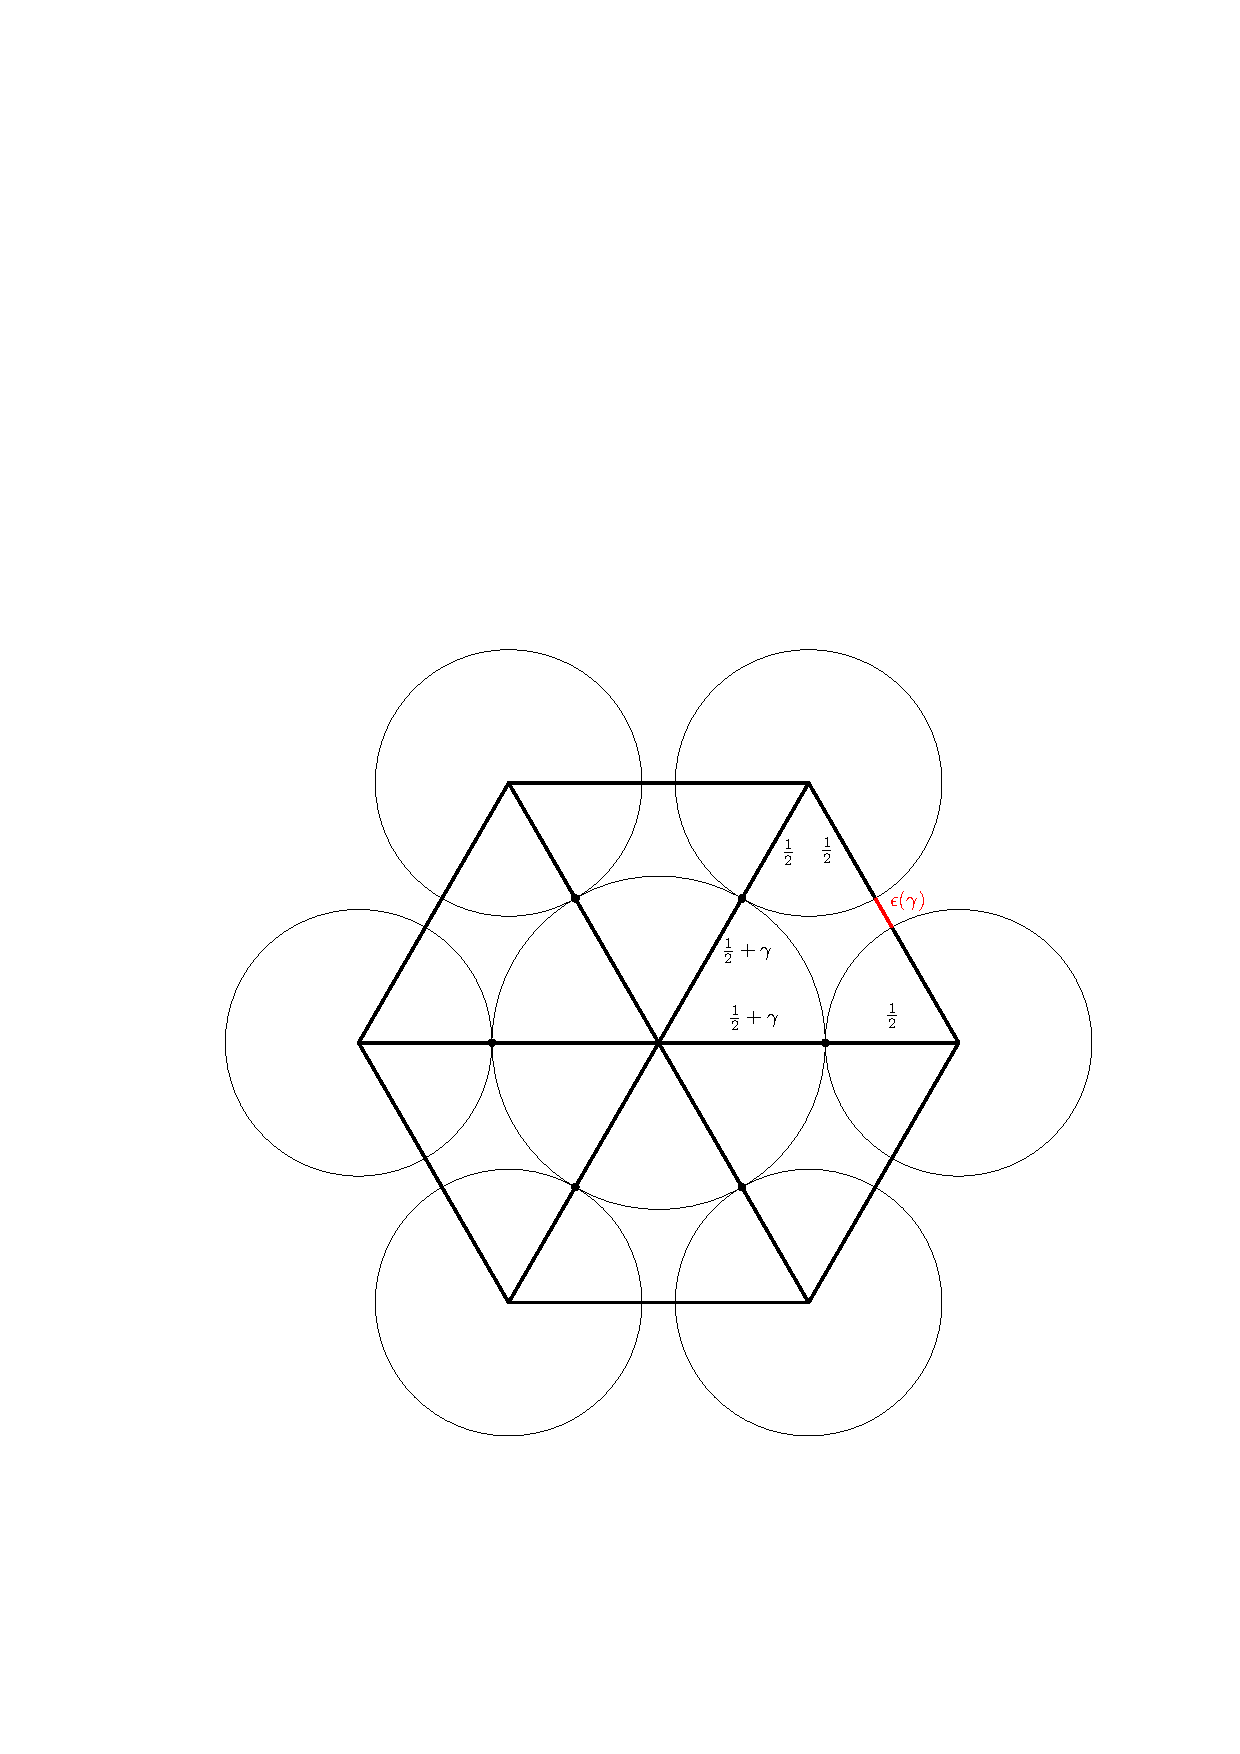
\includegraphics[width=.33\columnwidth]{graphics/modifiedContactGraph.pdf}
\captionof{figure}{A canonical disk arrangement from a perturbed snowflake with 6 unit disks around a central disk with radius $\frac{1}{2} + \gamma$.}\label{fig:modifiedContactGraph.pdf}
\end{center}
\end{minipage}

One way to do this is to demonstration that the sum of gaps for any realization of a contact graph of a perturbed snowflake $S_1$ is small. 
Denote the vertices around $v_0$ as $v_1$ through $v_6$ in a clockwise pattern about $v_0$. 
Without loss of generality, given a realization denote $\epsilon_{k, k+1} (\gamma)\geq 0$ as the gap created between adjacent disks corresponding to $v_1$ thourgh $v_6$.

Consider the realization where $\epsilon_{k, k+1} (\gamma) = 0$ with the exception of $\epsilon_{1,6} >0$.  
That is, ever consecutive pair of disks about the central disk is in contact with each other with the exception of $D_1$ and $D_6$.  
The realization provides 5 congruent triangles between the centers of $D_0$ and $\lr{D_1,D_2}$, $\lr{D_2,D_3}$, $\lr{D_3,D_4}$, $\lr{D_4,D_5}$, and $\lr{D_5,D_6}$.  
Given perturbation $\gamma > 0$, the side lengths between $\lr{D_0,D_i}$ are $1 +\gamma$ and the side length of $\lr{D_i, D_{i+1}}$ is 1.
Using law of cosine the angle formed between $\lr{D_0,D_i}$ and $\lr{D_0,D_{i+1}}$ is $$2 \tan^{-1} \frac{1}{2\lr{1+\gamma}}.$$  
The angle between $\lr{D_6, D_1}$ is $$y=2 \pi - 5 \cdot \lr{2 \tan^{-1} \frac{1}{2\lr{1+\gamma}}}.$$  
The side length of $\lr{D_6, D_1}$ is
$$\sqrt{-2 \, {\left(\gamma + 1\right)}^{2} \cos\left(-10 \,
\arctan\left(\frac{1}{2 \, {\left(\gamma + 1\right)}}\right)\right) + 2
\, {\left(\gamma + 1\right)}^{2}}.$$
Note that as $\gamma \rightarrow 0$, the side length of $\lr{D_6, D_1}$ is approximately 1 + .466861, where $\epsilon(\gamma) \approx .466861$ as $\gamma \rightarrow 0$.
This establishes an upperbound on the maximal displacement about $S_1$ with respect to the side lengths between the centers of disks about $D_0$.

The lower bound is established using the configuration found in Figure \ref{fig:modifiedContactGraph.pdf}.  
he realization provides 6 congruent triangles between the centers of $D_0$ and each disk about $D_0$.
Without loss of generality, to find the side length of between neighboring disks about $D_0$, we find need to $\epsilon(\gamma)$.  
The angle between $\lr{D_0, D_i}$ and $\lr{D_0,D_{i+1}}$ is $\frac{\pi}{3}$; using the law of cosine, we can determine the side length of $\lr{D_i,D_{i+1}}$ is $$\sqrt{1 + 2 \gamma + \gamma^2}.$$  


Thus the perturbation about $S_1$ in and confiugration is bounded and small.
\end{proof}
\subsection{Proof of Lemma \ref{lem:angularArrangement}}
\begin{proof}
Recall that we are to show that for any realized perturbed snowflake $S_i$, the angular value of $\alpha_k$ and $\beta_k$ are small.  
In canoncical position, the angle between $p_{k,j}^+$ and $p_{k,j}^-$ is $\frac{\pi}{3}$.  
In a non-canonical position, we define the change in angle to be $f(\epsilon)$.  
About a 
We prove this with induction. 


\begin{minipage}{\linewidth}
\begin{center}
\includegraphics[width=.66\columnwidth]{graphics/Vertebrae.pdf}
\captionof{figure}{}\label{fig:Vertebrae.pdf}
\end{center}
\end{minipage}

% First consider the changes the angles $\alpha_1$, $\beta_1$, $\alpha_2$, and $\beta_2$.  
$$
\begin{array}{rcl}
\alpha_i +\beta_i &\leq& 120 + f(\epsilon)\\
2 \pi &\leq& \gamma_i + \delta_i + \frac{2 \pi}{3} + f(\epsilon)\\
2 \pi - \lr{\gamma_i + \delta_i} &\leq& \frac{2 \pi}{3} + f(\epsilon)\\
\alpha_{i+1} + \beta_{i+1} &\leq& \frac{2 \pi}{3} + f(\epsilon)\\
\end{array}
$$
\end{proof}
\subsection{Proof of Lemma \ref{lem:disksOfPathways}}
\begin{proof}
Recall that we are to show that for any realized perturbed snowflake $S_i$, the distance between disks $D_{k,j}$, $D_{k+1,j}$, $D_{k+1,j+1}$, and $D_{k,j+1}$ are relatively small with respect to the relative distance in a perfect snowflake where $k = 1$, $\dots$, $6$ and $j = 2$, $\dots$, $i$.

\begin{minipage}{\linewidth}
\begin{center}
\includegraphics[width=.66\columnwidth]{graphics/ch4Paralellogram.pdf}
\captionof{figure}{}\label{fig:ch4Paralellogram.pdf}
\end{center}
\end{minipage}


\end{proof}
% ----------------------------
% CHAPTER 3. (Labels refer to the file cat.pdf)

% Glossary of formulas:
% For arctan, sin, cos, and sec, I would give upper and lower bounds
% (rather than approximate values).
% For example, the Maclaurin series of tan^{-1} gives: x-\frac{x}{3} <
% \tan^{-1}x < x for all 0<x<1.
% All lowerupper bounds are derived from the first or the first two terms
% of the Maclaurin series.


% In (3.5), I would simply (5s^\kappa-1)^3  to (4s^\kamma)^3=4s^{3\kappa},
% which is true for sufficiently large values of s (above a constant
% threshold).
% This will simplify the formulae (3.5)--(3.10).

% Below Figure 3.18, the paragraph title "Vertical Displacement delta" is
% missing.

% Below Figure 3.20. You introduce omega, but you later use omega_i.
% I would define omega_i from the start.

% Below Figure 3.21, you consider the case that omega_i \leq \pi/2.
% It is unclear why the threshold is \pi/2. Shouldn't it be
% \pi/2-2arctan(1/100N), that is \pi/2 minus twice the angle of
% angle of the right triangle shown in the bottom of Figure 3.21?

% Lemma 7, and the calculation above it: I don't understand this lemma.
% I think the main argument should something line this:
% --If omega_i is close to pi, then O_{i+1} has a horizontal displacement
% of about 2 units, and it
% overlaps with another obstacle (which has small displacement by induction).
% --If omega_i is between 0 and pi (but not close to either 0 or pi), then
%   the top vertex of the small rombus is "too high,", contradicting the
% fact the
%    O_{i+1} has "small" vertical displacement (here the terms "too high" and
%    "small" can be quantified in terms of the parameter s).

% -------------------------------------
% CHAPTER 4. OUTLINE

% In chapter 4, we show that for every epsilon>0 there exists an ordered
% weighted tree T_epsilon such that every realization of T_epsilon as an
% ordered disk contact graph, where the radii of the disks equal the
% vertex weights, has Housdorff distance at most epsilon 1 from a regular
% hexagon of unit side length. Once we establish this, we can prove
% Theorem 4 by extending the construction in Section 3 and simulating
% regular hexagons with ordered trees T_epsilon.

% Section 4.1 should define Hausdorff distance and eps-approximation; and
% provide a few examples.

% Section 4.2 should define the snowflake trees. It is an infinite family
% of ordered trees, say T_k,
% where teach axis contains k vertices.

% Section 4.3 should show that for every k, the snowflake tree (with
% vertex weights 1/2+delta and 1/2
% can be realized as a contact graph of disks; and this realization has
% Hausdorff distance at most 1
% from a regular Hexagon (of side length k). Let us also define a
% "canonical position" of the disk
% centers; where each center is a vertex of the hexagonal lattice. Note,
% however, that the canonical
% position does not give a valid realization!

% Section 4.4 should prove that in  _every_ realization of the snowflake
% tree T_k, every disks is "close"
% to their canonical position (here the term "close" must be
% quantified---an upper bound on the maximal distance of a disk from its
% canonical position comes from the proof).

% Section 4.5: Proof of Theorem 4 (this should be rather short: we simply
% state that the construciton of Section 3 can be repeated).

% -----------------------------------
% Lemma 1 in Chapter 4.

% The statement of the lemma is fine, just need to quantify it in terms of
% gamma.

% In the proof of the lemma, the formula
% y = 2\pi - 5( 2 \tan^{-1} frac{1}{2(1+gamma)}
%    = 2\pi - 10 \tan^{-1} frac{1}{2(1+gamma)}
% is great. Observe that if gamma=0, then y=pi/3.
% By continuity, for small values of gamma,
% y will be close to pi/3.

% Note that 1-1/(1+gamma) < gamma.
% Since the derivative of tan^{-1}(x) is less than 1;
% we conclude that  tan^{-1} frac{1}{2(1+gamma)}
% < tan^{-1}(frac{1}{2})  + frac{1}{2}(1-frac{1}{1+ gamma}
% < pi/3 + gamma/2.
% -----------------------------------

% Caterpillar concept:

% A caterpillar can simulate a small rhombus.

% But the main point is Lemma 2 in that paper, which can be used directly
% for the proof of Lemma 2 in Chapter 4 (to show the displacement is small
% for every axis of the snowflake graph. .

% -------------------------------------